\begin{Minutes}{Status Update and Next Steps Discussion}
%%\subtitle{}
%%\moderation{}
%%\minutetaker{}
\participant{Daniel Cizin, David Knowles, Stephen Malina}
%%\missingExcused{}
%%\missingNoExcuse{}
\minutesdate{January 29, 2020}
%%\starttime{}
%%\endtime{}
%%\cc{}
\maketitle
We discussed a few topics:
\begin{enumerate}
    \item Getting standard error estimates from NN predictions.
    \item Inverse variance weighted methods for conducting meta-analyses.
    \item How to do in-silico mutation such that we don't condition on the exposure and also get effects we can combine.
\end{enumerate}

Summarizing our decisions in order of dependency rather than chronologically:
\begin{enumerate}
    \item At least for now, we're going to try and get results from the ``multiple DAG instantiations with mutations as IVs'' framework.
    \item High-level our strategy will be:
        \begin{itemize}
            \item randomly sample sequences;
            \item do saturation mutagenesis for each, getting a standard error for each mutation's prediction;
            \item run Egger (or similar, e\.g\., RAPS) on the result for each sequence, treating the difference between the binding probability for the mutated and wild type sequences as an effect size; and
            \item combine the causal estimates for each sequence together using a meta-analysis protocol.
        \end{itemize}
    \item For getting standard errors for individual predictions, we'll using Yarin Gal's method of repeated dropout.
    \item We hope that using a robust regression method will allow us to get an estimate of how much violation of exclusion-restriction there is in our model.
\end{enumerate}

Given this, our follow-ups are:
\task{Stephen}{Verify that with classification, we don't care about the noise variables in the prediction variance formula.}
\task{Stephen}{Figure out and implement the saturation mutagenesis with uncertainty estimates logic on top of Kipoi.}
\task{Daniel}{Do some research into how likely it seems that sequence will influence accessibility directly.}
\task{Daniel}{Try and understand the difference between Egger regression and RAPS.}
\task*{Keep thinking about the idea of using cell type, potentially in a deep IV framework, as an alternative IV.}
\task*{Keep thinking about whether there's something interesting in investigating the covariance betwen predictions from saturation mutagenesis (see figure~\ref{fig:2}).}

On the next page, I put the two pictures I took of the whiteboard during our meeting.
\begin{figure}[h]
    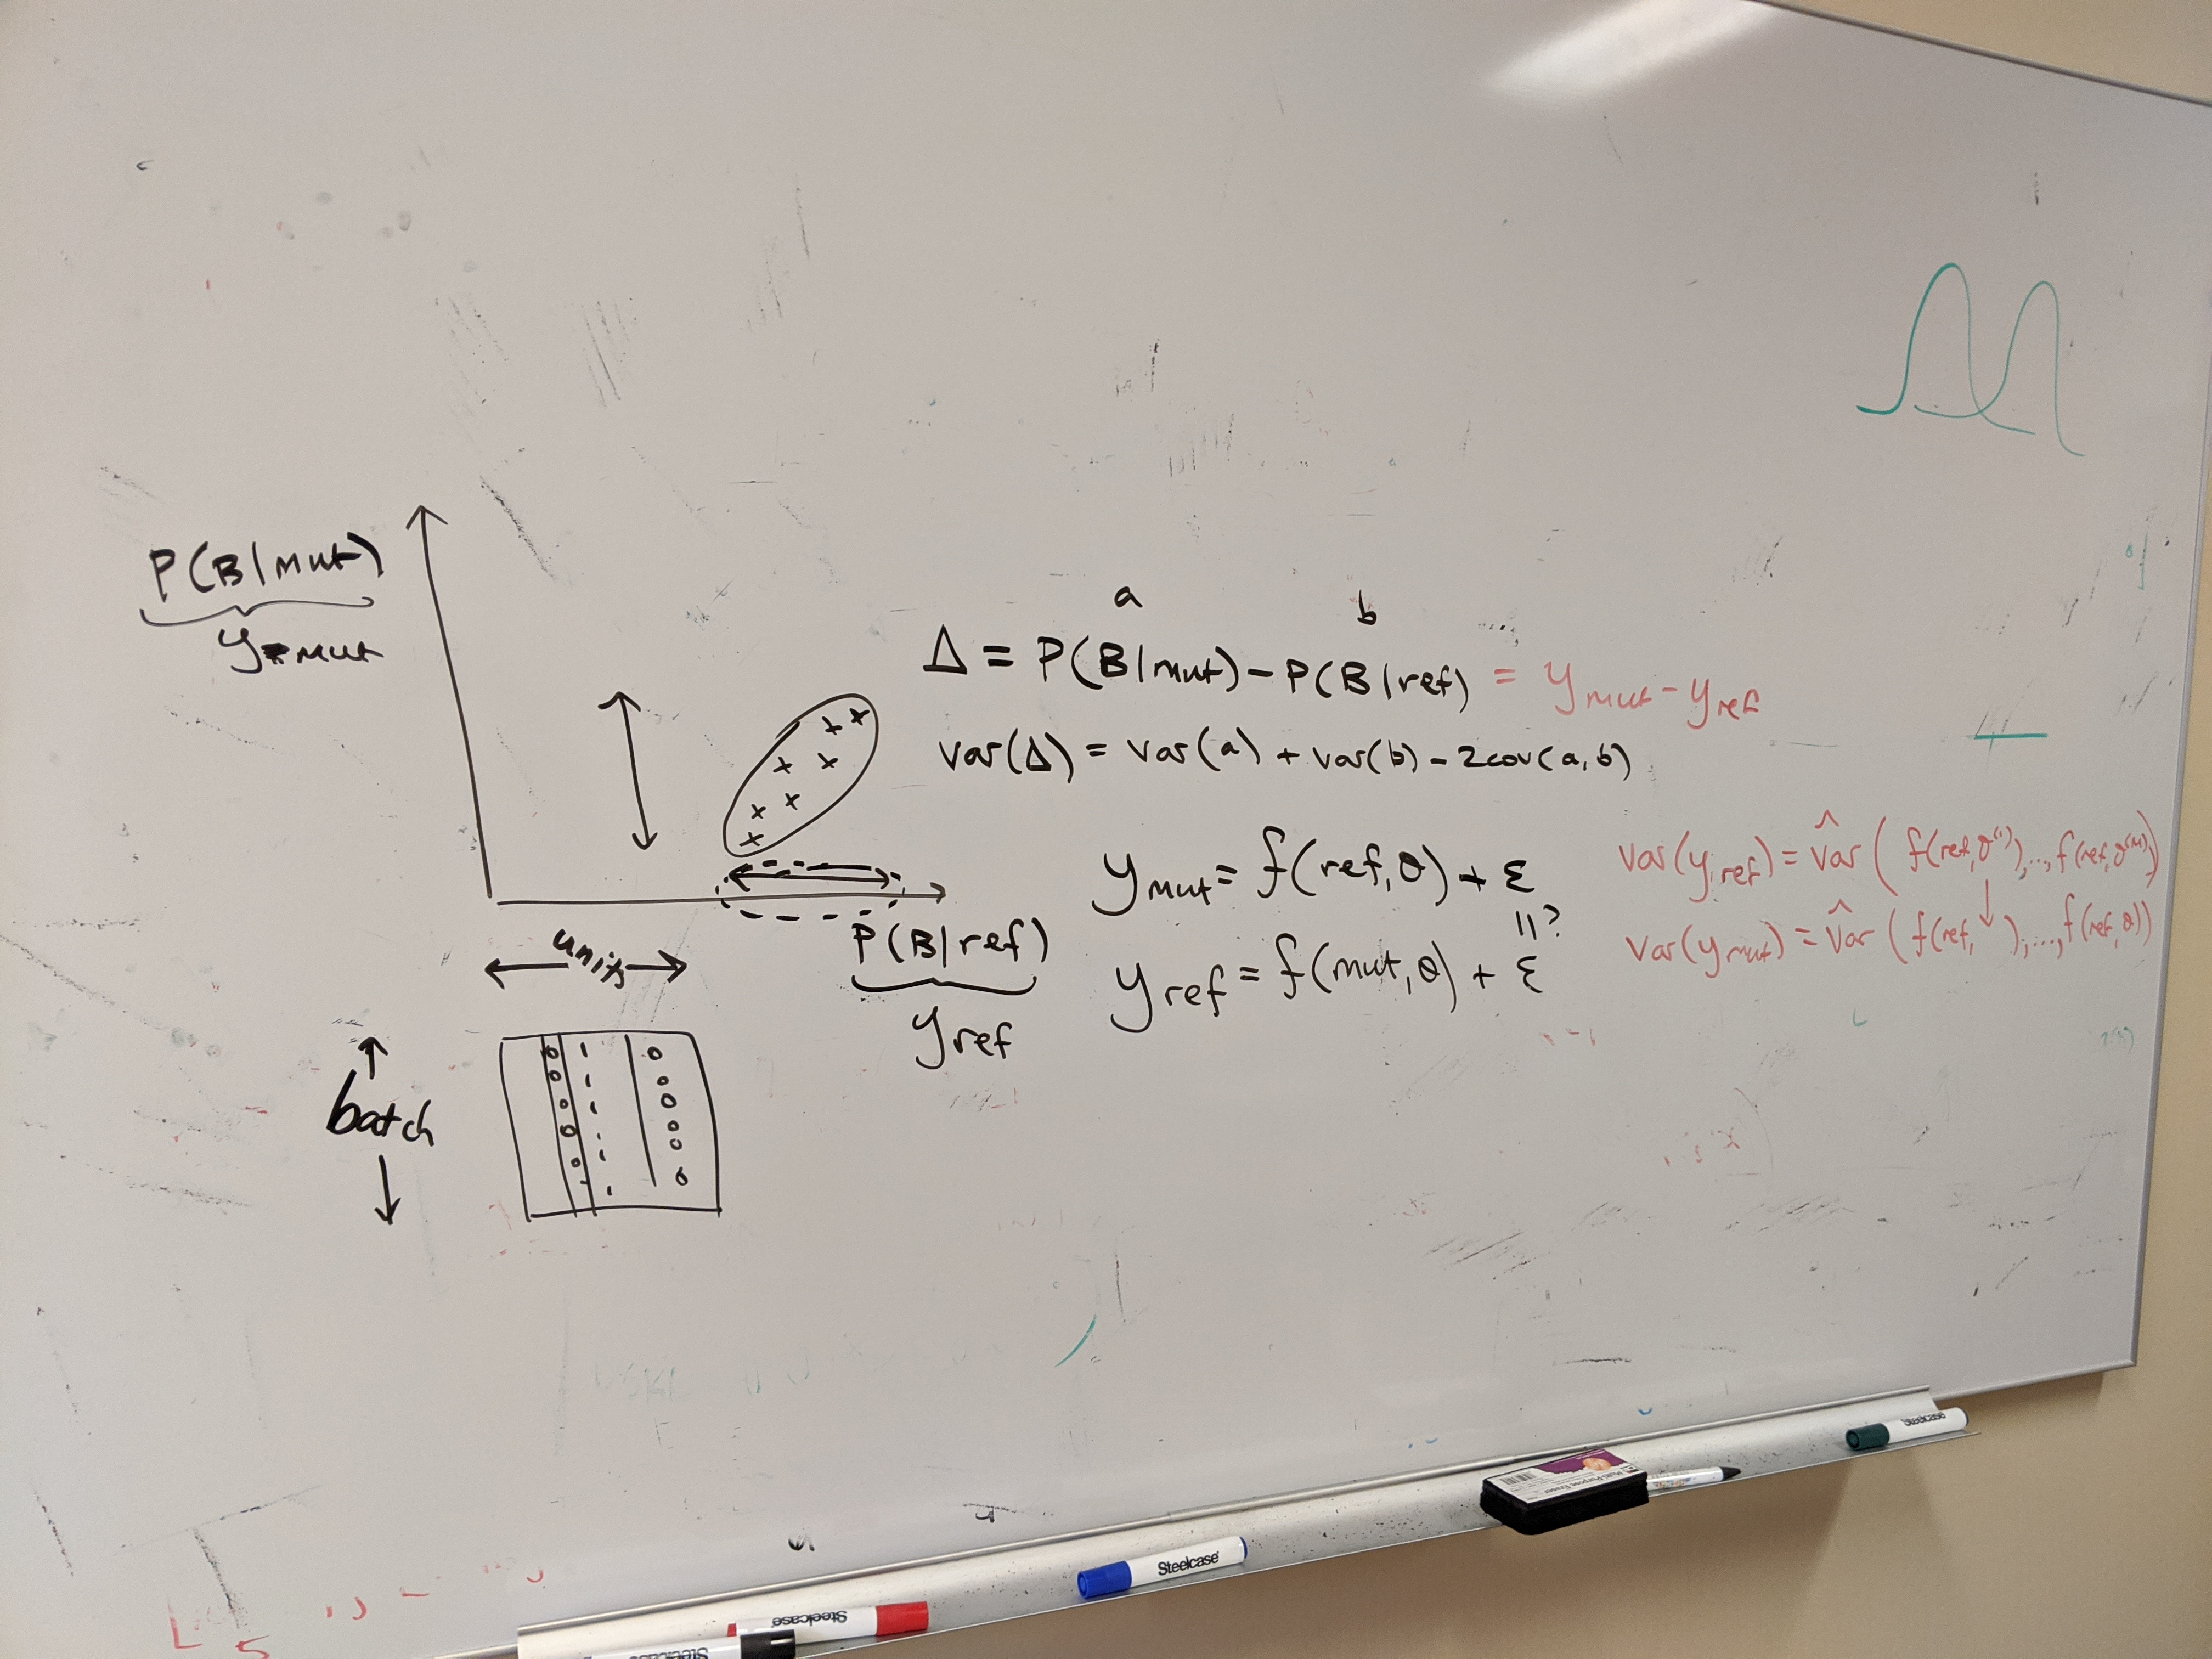
\includegraphics[width=.9\textwidth]{figures/whiteboard_20200129_1}
    \caption{Shows two things: that we should take the std error of the diff between mut and wild type probabilities and that we want to use the same dropout mask for mut and wild type predictions so that we can estimate the covariance between the two.}
\end{figure}
\begin{figure}[h]
    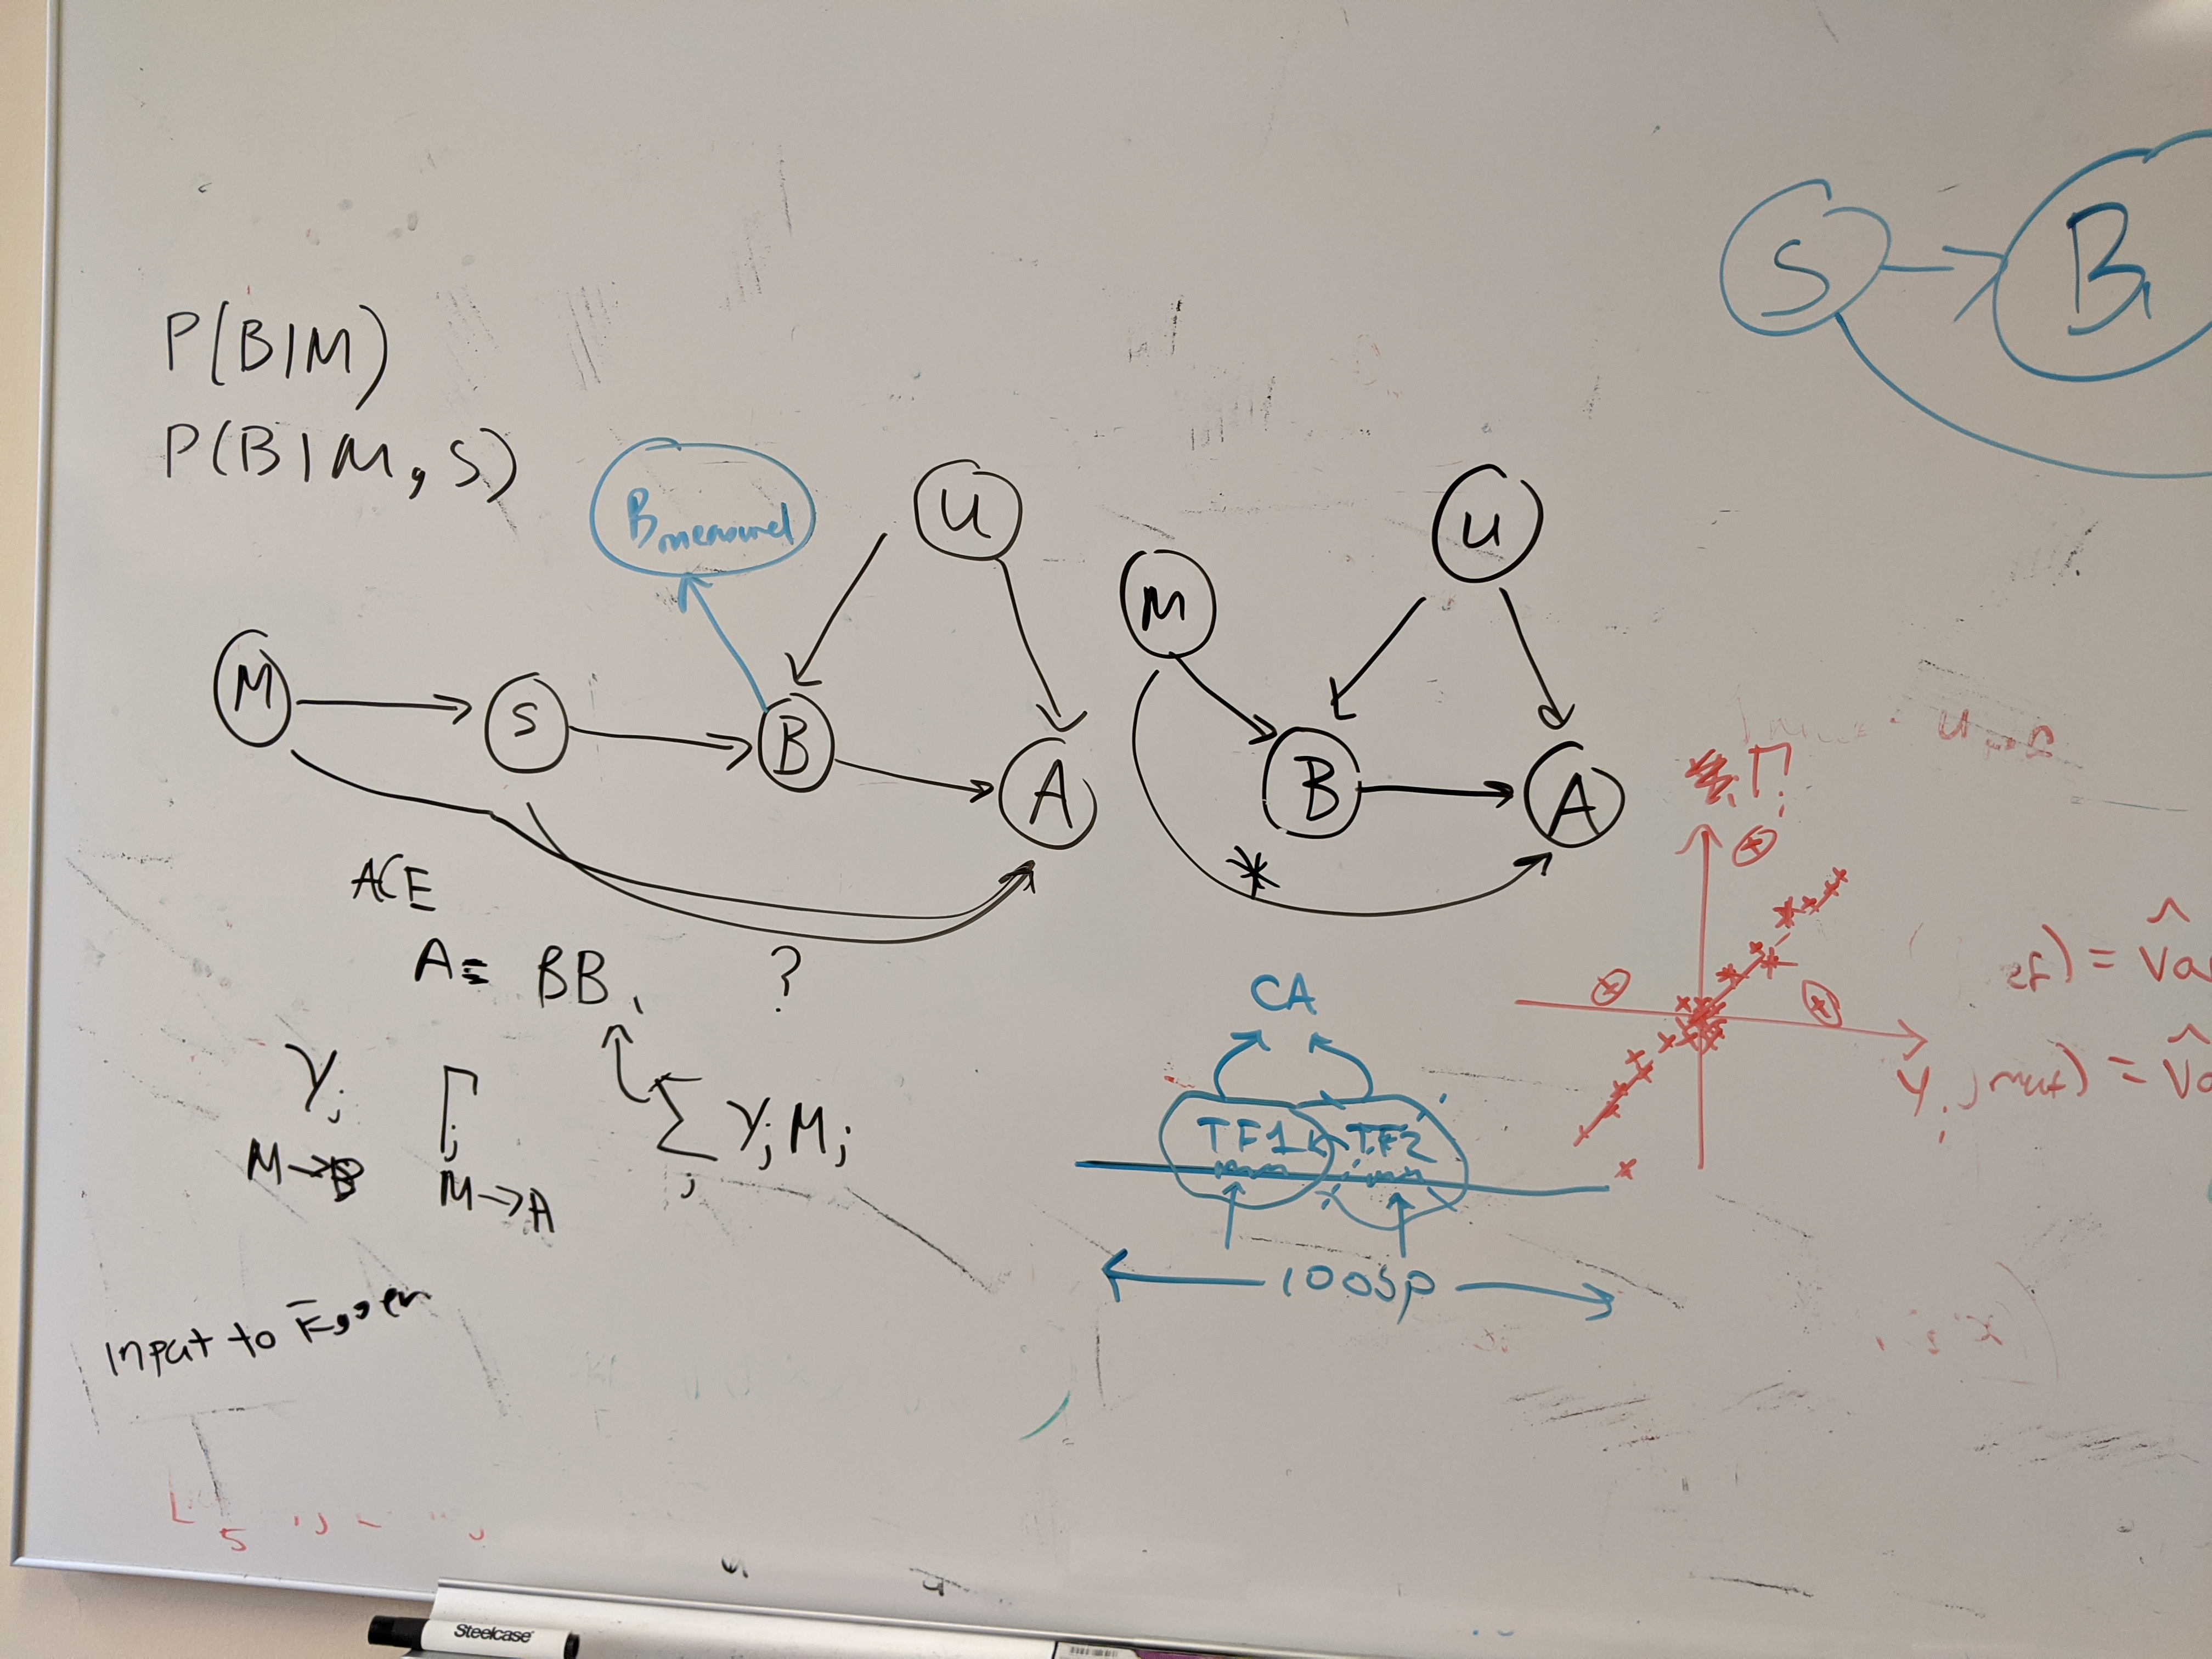
\includegraphics[width=.9\textwidth]{figures/whiteboard_20200129_2}
    \caption{Captures two notable things. First, that we mostly came to the conclusion that because of potential exclusion restriction violations, it makes to analyze the causal effect separately for each sequence and then aggregate. Second, that there may be something interesting in the covariance between different mutation predictions for the same sequence.}
    \label{fig:2}
\end{figure}

\end{Minutes}
